\chapter{Funciones de onda del oscilador, espín uno medio e intercambio de partículas}

\section{Osciladores por todas partes}

Todo sistema con un equilibrio estable puede oscilar si se lo desplaza de ese equilibrio. Puede tener una frecuencia o muchas. Por ejemplo, una cuerda de violín tiene un modo fundamental y armónicos superiores. Al pulsarla, se excita una combinación de esos modos.

Aquí, los ejemplos más importantes son los campos. La configuración de equilibrio del campo electromagnético es el vacío: no hay campo eléctrico, campo magnético ni oscilación electromagnética. Si se introduce radiación en una cavidad o una guía de ondas, el campo puede oscilar en sus modos permitidos, cada uno con su propia frecuencia. En la teoría cuántica, esos modos describen conjuntos de fotones.

La misma idea se aplica a un cristal. Es engañoso imaginar cada átomo como un oscilador independiente. Los átomos ejercen fuerzas unos sobre otros, así que el desplazamiento de un átomo afecta a sus vecinos y una onda se propaga por el cristal. Los modos normales de ese movimiento acoplado son osciladores armónicos, y sus cuantos se llaman fonones. Los fotones y los fonones son objetos físicos distintos, pero ambos conducen a la misma álgebra del oscilador.

\section{El álgebra del oscilador}

Para estudiar el oscilador, igualemos a uno la masa y la constante de Planck reducida:
\[
m=1,\qquad \hbar=1.
\]
El hamiltoniano es
\begin{equation}
H=\frac{p^{2}}{2}+\frac{\omega^{2}x^{2}}{2}.
\end{equation}
El parámetro \(\omega\) determina la curvatura del potencial y también es la frecuencia de oscilación.

Definamos los operadores de subida y bajada mediante
\begin{equation}
A_{\pm}=\frac{p\pm i\omega x}{\sqrt{2\omega}}.
\end{equation}
La normalización se elige de modo que
\begin{equation}
[A_{-},A_{+}]=1.
\end{equation}
El operador número es
\begin{equation}
N=A_{+}A_{-}.
\end{equation}
En conjunto, estas ecuaciones implican que \(A_{+}\) aumenta en una unidad un autovalor de \(N\) y que \(A_{-}\) lo disminuye en una unidad. El espectro resultante es
\begin{equation}
n=0,1,2,3,\ldots .
\end{equation}

El producto de los dos operadores escalera también pone de manifiesto la corrección cuántica a la energía clásica:
\begin{align}
N
&=\frac{1}{2\omega}(p+i\omega x)(p-i\omega x)\\
&=\frac{1}{2\omega}\left(p^{2}+\omega^{2}x^{2}
 +i\omega[x,p]\right)\\
&=\frac{1}{2\omega}\left(p^{2}+\omega^{2}x^{2}-\omega\right),
\end{align}
donde \([x,p]=i\). Por consiguiente,
\begin{equation}
H=\omega\left(N+\frac12\right).
\end{equation}
Si la constante aditiva no es relevante para el problema, resulta conveniente usar el hamiltoniano desplazado
\begin{equation}
H_{\mathrm{shifted}}=H-\frac{\omega}{2}=\omega N.
\end{equation}
El término \(\omega/2\) es la energía de punto cero, o energía del estado fundamental, del oscilador. Para un modo del campo, el término análogo se llama energía del vacío. Refleja el principio de incertidumbre: ningún estado puede tener \(x\) y \(p\) ambos exactamente iguales a cero, así que los dos términos cuadráticos positivos de \(H\) no pueden tener simultáneamente valor esperado nulo.

\begin{classroomqa}
\lecturetimestamp{00:09:46}
\audiencequestion{¿Por qué el cero está incluido en el espectro del operador número?}
\lecturerresponse{Se puede demostrar explícitamente construyendo la función de onda del estado fundamental. Esa construcción mostrará un estado con \(N=0\).}
\end{classroomqa}

Para empezar esa construcción, sustituyamos los vectores de estado por funciones de onda en la representación de posición. Los estados propios de energía pasan a ser
\[
\psi_{0}(x),\ \psi_{1}(x),\ \psi_{2}(x),\ldots,
\]
y los operadores básicos actúan como
\begin{equation}
X\longmapsto x,\qquad
P\longmapsto -i\frac{d}{dx}.
\end{equation}
Al restituir \(\hbar\), la segunda sustitución sería
\(P\mapsto-i\hbar\,d/dx\).

Antes de resolver para \(\psi_{0}\), hay una respuesta abstracta más rápida a la pregunta. En la escalera discreta de estados propios normalizables del oscilador, \(N=A_{+}A_{-}\) es no negativo, así que no se puede seguir bajando repetidamente en pasos unitarios de manera indefinida. En el extremo---cuya función de onda normalizable se construirá más adelante---debe haber un estado, denotado \(\lvert0\rangle\), para el cual
\begin{equation}
A_{-}\lvert0\rangle=\mathbf 0.
\end{equation}
De lo contrario, \(A_{-}\lvert0\rangle\) sería otro estado un escalón más abajo. De ello se sigue inmediatamente que
\begin{equation}
N\lvert0\rangle
=A_{+}A_{-}\lvert0\rangle
=\mathbf 0
=0\,\lvert0\rangle.
\end{equation}
Por tanto, el estado más bajo tiene autovalor cero del operador número.

\begin{classroomqa}
\lecturetimestamp{00:14:57}
\audiencequestion{Si el autovalor es cero, ¿no debería aparecer a la derecha un vector propio nulo?}
\lecturerresponse{El ket \(\lvert0\rangle\) es un vector normalizado, distinto de cero, cuyo rótulo es cero. En \(N\lvert0\rangle=0\,\lvert0\rangle\), el miembro derecho es el vector nulo. El ket del estado fundamental y el vector nulo son objetos distintos.}
\end{classroomqa}

\section{La ecuación de Schr\"odinger y las soluciones físicas}

Volvamos ahora a la representación de posición. La ecuación de Schr\"odinger independiente del tiempo es
\begin{equation}
\left[
-\frac12\frac{d^{2}}{dx^{2}}
+\frac12\omega^{2}x^{2}
\right]\psi(x)=E\psi(x).
\end{equation}
Como ecuación diferencial de segundo orden, tiene soluciones formales para valores arbitrarios de \(E\). La mayoría de esas soluciones formales no corresponden a estados físicos del oscilador. Crecen exponencialmente cuando \(\lvert x\rvert\) es grande, por lo que su norma diverge.

Para un estado ligado, la función de onda debe ser de cuadrado integrable:
\begin{equation}
\int_{-\infty}^{\infty}\psi^{*}(x)\psi(x)\,dx<\infty.
\end{equation}
Entonces se puede normalizar para que la integral sea igual a uno. Solo ciertos valores especiales de la energía producen soluciones de ese tipo. Los estados de posición y de momento en una recta infinita son excepciones en este sentido, pero las soluciones del oscilador que crecen exponencialmente simplemente se excluyen del espacio de estados.

\section{El estado fundamental gaussiano}

La ecuación de segundo orden se puede resolver, pero el álgebra de los operadores escalera conduce a una ecuación más sencilla, de primer orden:
\begin{equation}
A_{-}\psi_{0}(x)=0.
\end{equation}
El factor global de \(A_{-}\) es irrelevante cuando el miembro derecho es cero, así que esto equivale a
\begin{equation}
(p-i\omega x)\psi_{0}(x)=0.
\end{equation}
Usando \(p=-i\,d/dx\) se obtiene
\begin{equation}
\left(\frac{d}{dx}+\omega x\right)\psi_{0}(x)=0.
\end{equation}

\begin{classroomqa}
\lecturetimestamp{00:22:32}
\audiencequestion{¿Se podría resolver esto mediante separación de variables?}
\lecturerresponse{Solo hay una variable independiente, así que no hay dos variables que separar. Escrita como \(\psi_{0}'/\psi_{0}=-\omega x\), la ecuación tiene la forma de una derivada logarítmica. Eso sugiere expresar la función de onda como una exponencial.}
\end{classroomqa}

Una forma útil de resolverla es escribir
\begin{equation}
\psi_{0}(x)=e^{f(x)}.
\end{equation}
Entonces
\[
\psi_{0}'(x)=f'(x)e^{f(x)},
\]
y el factor exponencial común se cancela. La ecuación se reduce a
\begin{equation}
\frac{df}{dx}+\omega x=0.
\end{equation}

\begin{classroomqa}
\lecturetimestamp{00:26:28}
\audiencequestion{¿Debería haber un signo menos en \(f(x)\)?}
\lecturerresponse{Sí. Puesto que \(df/dx=-\omega x\), la integración da un término cuadrático negativo.}
\end{classroomqa}

Por tanto,
\begin{equation}
f(x)=-\frac12\omega x^{2}+C,
\end{equation}
y
\begin{equation}
\psi_{0}(x)\propto e^{-\omega x^{2}/2}.
\end{equation}
La constante multiplicativa de normalización queda sin especificar. Lo importante es la forma gaussiana: es suave, está concentrada cerca del origen y decrece rápidamente cuando aumenta \(\lvert x\rvert\). Claramente es de cuadrado integrable.

No hace falta sustituir la respuesta en la ecuación de segundo orden para hallar su energía. El álgebra ya da
\begin{equation}
E_{0}=\frac{\omega}{2}.
\end{equation}

\section{Estados excitados, nodos y movimiento clásico}

El primer estado excitado se obtiene aplicando el operador de subida al estado fundamental:
\begin{equation}
\psi_{1}(x)\propto A_{+}\psi_{0}(x)
\propto(p+i\omega x)e^{-\omega x^{2}/2}.
\end{equation}
La ecuación del estado fundamental dice que
\[
p\psi_{0}=i\omega x\,\psi_{0}.
\]
Cambiar el signo en el operador escalera convierte la cancelación en una suma:
\begin{equation}
(p+i\omega x)\psi_{0}
=2i\omega x\,\psi_{0}.
\end{equation}
Salvo una constante global,
\begin{equation}
\psi_{1}(x)\propto x\,e^{-\omega x^{2}/2}.
\end{equation}

Esta función de onda es impar:
\begin{equation}
\psi_{1}(-x)=-\psi_{1}(x).
\end{equation}
Su densidad de probabilidad es par, pero tiene un nodo en el origen,
\begin{equation}
\lvert\psi_{1}(0)\rvert^{2}=0.
\end{equation}
Así, la densidad de probabilidad del primer estado excitado tiene un nodo en \(x=0\).

La acción repetida de \(A_{+}\) produce polinomios de grado creciente que multiplican la misma envolvente gaussiana.\footnote{La exposición indica los factores polinómicos de grado creciente, el nodo adicional en cada paso y la simetría alternante entre \(00{:}34{:}25\) y \(00{:}35{:}49\). La forma de producto de una gaussiana por un polinomio también está corroborada por Leonard Susskind y Art Friedman, \emph{Mecánica cuántica: el mínimo teórico} (2014), en su análisis de las funciones propias del oscilador.} Salvo normalización,
\begin{equation}
\psi_{n}(x)=P_{n}(x)e^{-\omega x^{2}/2}.
\end{equation}
La paridad alterna entre par e impar, y en cada paso se añade un nodo. A medida que aumenta \(n\), la función de onda se extiende más lejos del origen y presenta oscilaciones más rápidas.

Las dos características tienen significados físicos directos. Una mayor extensión lejos del origen corresponde a una energía potencial mayor, porque el potencial crece como \(x^{2}\). Las oscilaciones rápidas en el espacio de posiciones indican un momento mayor. Es probable que un oscilador muy excitado llegue más lejos del centro; al pasar por la región central, lleva un momento mayor y su función de onda oscila más rápidamente allí.

\begin{classroomqa}
\lecturetimestamp{00:37:18}
\audiencequestion{¿Deja el oscilador armónico de aproximarse al comportamiento clásico cuando \(n\) se hace grande?}
\lecturerresponse{El movimiento clásico no está representado por un único estado propio estacionario de energía. Aparece en un paquete de ondas que contiene muchos niveles de energía. Por ejemplo, un paquete gaussiano desplazado evoluciona de un lado a otro como un oscilador clásico, y la incertidumbre relativa disminuye a medida que aumenta la amplitud de la oscilación.}
\end{classroomqa}

Partamos de la gaussiana del estado fundamental y desplacémosla respecto del origen. El paquete desplazado ya no es un estado propio de energía: es una superposición de muchos estados propios. Según la ecuación de Schr\"odinger dependiente del tiempo, sus componentes adquieren fases distintas. El paquete oscila de un lado del potencial al otro, desarrolla una variación rápida de fase cerca del centro y vuelve a hacerse suave cerca de un punto de retorno. Cuanto mayor sea la excursión en comparación con la anchura del paquete, más clásico parecerá el movimiento.

\begin{classroomqa}
\lecturetimestamp{00:39:29}
\audiencequestion{¿Debería anularse en el origen la función de onda del segundo estado excitado?}
\lecturerresponse{No. Su factor polinómico no es simplemente \(x^{2}\); también contiene un término constante, así que la función de onda no tiene por qué anularse en \(x=0\).}
\end{classroomqa}

El argumento de los operadores escalera también supone que \(A_{+}\) y \(A_{-}\) son adjuntos hermíticos en el dominio de funciones de cuadrado integrable del oscilador, con el comportamiento en los bordes necesario para que se cumpla la relación de adjunción. Las soluciones formales que crecen exponencialmente no pertenecen a ese dominio.

\begin{classroomqa}
\lecturetimestamp{00:40:45}
\audiencequestion{¿Hay alguna forma general de reconocer cuándo se puede resolver un hamiltoniano con estos métodos algebraicos?}
\lecturerresponse{No hay una regla general de ese tipo. Los ejemplos exactamente solubles son escasos. El oscilador armónico y el átomo de hidrógeno no relativista ideal son casos afortunados en los que funcionan los métodos algebraicos.}
\end{classroomqa}

\section{El espín uno medio como momento angular}

El espín es un momento angular que lleva una partícula independientemente de su movimiento orbital respecto del centro de masa. Una partícula en reposo no tiene momento angular orbital \(\mathbf R\times\mathbf P\), pero aún puede tener espín. Se puede intentar imaginar un objeto diminuto que gira, o tratar el espín como una propiedad cuántica intrínseca. La afirmación decisiva es matemática: sus componentes se transforman bajo rotaciones espaciales y obedecen las relaciones de conmutación del momento angular.

A partir de aquí, restituyamos \(\hbar\). Las componentes del momento angular satisfacen
\begin{equation}
[L_{z},L_{x}]=i\hbar L_{y},
\end{equation}
y las otras dos relaciones se obtienen mediante permutaciones cíclicas. Las matrices de Pauli adimensionales son
\begin{equation}
\begin{aligned}
\sigma_{z}&=
\begin{pmatrix}
1&0\\
0&-1
\end{pmatrix},\\[0.4em]
\sigma_{x}&=
\begin{pmatrix}
0&1\\
1&0
\end{pmatrix},\\[0.4em]
\sigma_{y}&=
\begin{pmatrix}
0&-i\\
i&0
\end{pmatrix}.
\end{aligned}
\end{equation}
En esta base, \(\sigma_{z}\) es diagonal. Sus autovalores son \(+1\) y
\(-1\).

\begin{classroomqa}
\lecturetimestamp{00:47:35}
\audiencequestion{¿Hay un signo menos en \(\sigma_x\)?}
\lecturerresponse{No. Las dos entradas no diagonales de \(\sigma_x\) son positivas.}
\end{classroomqa}

El cálculo en la pizarra en \(00{:}49{:}35\) inicia la multiplicación elemento por elemento. Al completar los productos se obtiene
\begin{align}
\sigma_{z}\sigma_{x}
&=
\begin{pmatrix}
0&1\\
-1&0
\end{pmatrix}
=i\sigma_{y},\\
\sigma_{x}\sigma_{z}
&=
\begin{pmatrix}
0&-1\\
1&0
\end{pmatrix}
=-i\sigma_{y}.
\end{align}
Por tanto,
\begin{equation}
[\sigma_{z},\sigma_{x}]=2i\sigma_{y}.
\end{equation}
El factor adicional de dos se elimina definiendo los operadores físicos de espín como\footnote{En el cálculo de la pizarra se omite \(\hbar\). Aquí se restituye para que \(S_i\) tenga unidades de momento angular.}
\begin{equation}
S_{i}=\frac{\hbar}{2}\sigma_{i}.
\end{equation}
Entonces
\begin{equation}
[S_{z},S_{x}]=i\hbar S_{y},
\end{equation}
y análogamente para las permutaciones cíclicas. Por tanto, la mitad de las matrices de Pauli, con el factor de \(\hbar\) restituido, constituye un sistema de momento angular.

Al fijar \(\hbar=1\) se obtiene la forma que se muestra a continuación.\footnote{El fotograma de origen es \texttt{\_04\_\_02}.}
\begin{figure}[htbp]
\centering
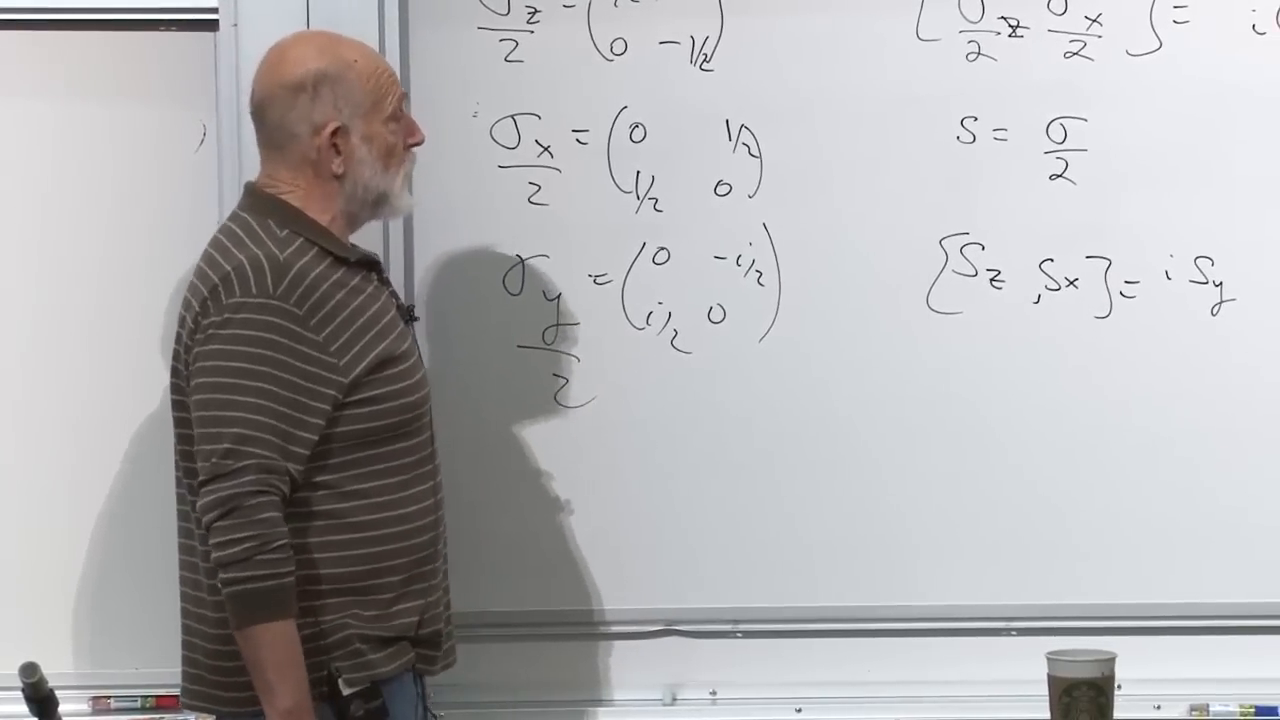
\includegraphics[width=0.9\linewidth]{lecture_04_frame_02.png}
\caption{En unidades en las que \(\hbar=1\), la mitad de las matrices de Pauli son los operadores de momento angular de espín uno medio y satisfacen \([S_z,S_x]=iS_y\).}
\lectureframe{00:55:41}
\end{figure}

Las dos ecuaciones de autovalores de \(S_z\) son
\begin{equation}
S_z\lvert\pm\rangle
=\pm\frac{\hbar}{2}\lvert\pm\rangle.
\end{equation}
Equivalentemente, el número cuántico magnético adimensional es
\begin{equation}
m_{s}=\pm\frac12,
\qquad
S_{z}\lvert m_{s}\rangle
=m_{s}\hbar\,\lvert m_{s}\rangle.
\end{equation}
Los operadores de subida y bajada del momento angular desplazan \(m\) en pasos enteros, pero esto no exige que todas las escaleras pasen por cero. Los multipletes de espín entero contienen valores enteros de \(m\), mientras que los multipletes de espín semientero contienen valores semienteros. Para el espín uno medio, la escalera tiene solo los dos estados \(m_s=+1/2\) y \(m_s=-1/2\).

Estos dos estados forman el doblete de espín uno medio. Los electrones, muones, neutrinos y quarks se cuentan entre las partículas descritas por multipletes de espín semientero.

\section{Momento angular orbital y de espín}

Ahora hay dos tipos de momento angular. El momento angular orbital describe el movimiento respecto de un origen,
\begin{equation}
\mathbf L=\mathbf R\times\mathbf P,
\end{equation}
mientras que \(\mathbf S\) es espín intrínseco. Su suma vectorial es el momento angular total,
\begin{equation}
\mathbf J=\mathbf L+\mathbf S.
\end{equation}

\begin{classroomqa}
\lecturetimestamp{00:56:49}
\audiencequestion{Si un sistema tiene momento angular total \(\mathbf J\), ¿cómo se identifica su espín \(\mathbf S\)?}
\lecturerresponse{Por lo general, los números cuánticos de espín y orbital se especifican por separado. Si \(L=0\), todo el momento angular es espín. De lo contrario, se necesitan las reglas cuánticas para sumar momentos angulares, que se dejan para más adelante.}
\end{classroomqa}

Las reglas de suma se aplican por igual al momento angular orbital más el espín, a dos espines o a dos momentos angulares orbitales. El sistema combinado tiene sus propios valores permitidos de momento angular total, pero aún no hacen falta esas reglas.

\begin{classroomqa}
\lecturetimestamp{00:58:18}
\audiencequestion{¿Qué evidencia experimental llevó a introducir el espín?}
\lecturerresponse{La espectroscopia aportó evidencia, pero la tabla periódica ofrece una motivación particularmente clara: su estructura de capas exige que los electrones tengan una propiedad adicional de dos valores.}
\end{classroomqa}

\section{Degeneración hidrogenoide y conteo de capas}

Para el momento angular orbital, la ecuación de autovalores de \(L^{2}\) es
\begin{equation}
L^{2}\lvert\ell,m\rangle
=\hbar^{2}\ell(\ell+1)\lvert\ell,m\rangle,
\end{equation}
y un valor fijo de \(\ell\) tiene
\begin{equation}
2\ell+1
\end{equation}
estados magnéticos, correspondientes a \(m=-\ell,-\ell+1,\ldots,\ell\).

El problema de Coulomb no relativista ideal presenta una degeneración adicional. Las energías de los estados ligados son negativas y se acercan a cero desde abajo, pero para el conteo solo importa cómo se alinean los niveles. El primer nivel \(\ell=1\) se alinea con el siguiente nivel \(\ell=0\); el primer nivel \(\ell=2\) se suma a la siguiente capa principal, y el patrón continúa.\footnote{\texttt{\_04\_\_03}, \(01{:}02{:}01\); la alineación completa de las capas principales se indica desde \(01{:}02{:}33\) hasta \(01{:}04{:}10\).}

\begin{figure}[htbp]
\centering
\begin{tikzpicture}[x=1.55cm,y=1.0cm]
\draw[->] (-0.65,0) -- (-0.65,4.35);
\draw[->] (-0.85,0) -- (4.75,0);
\node at (-0.95,4.08) {\(E\)};
\node at (4.55,-0.28) {\(\ell\)};
\node at (0,-0.30) {\(0\)};
\node at (2,-0.30) {\(1\)};
\node at (4,-0.30) {\(2\)};

\draw (-0.20,0.75) -- (0.20,0.75);

\draw (-0.20,2.00) -- (0.20,2.00);
\foreach \dx in {-0.18,0,0.18}
  \draw (2+\dx-0.06,2.00) -- (2+\dx+0.06,2.00);

\draw (-0.20,3.15) -- (0.20,3.15);
\foreach \dx in {-0.18,0,0.18}
  \draw (2+\dx-0.06,3.15) -- (2+\dx+0.06,3.15);
\foreach \dx in {-0.32,-0.16,0,0.16,0.32}
  \draw (4+\dx-0.05,3.15) -- (4+\dx+0.05,3.15);

\node[anchor=west] at (0.35,0.75) {\(n=1\)};
\node[anchor=west] at (2.35,2.00) {\(n=2\)};
\node[anchor=west] at (4.40,3.15) {\(n=3\)};
\end{tikzpicture}
\caption{Las tres primeras capas de Coulomb ideales combinan multipletes orbitales con la misma energía principal: un estado en la primera capa, \(1+3\) en la segunda y \(1+3+5\) en la tercera.}
\lectureframe{01:02:01}
\end{figure}

En la capa principal \(n\), los valores orbitales permitidos son\footnote{Este intervalo compacto de \(\ell\) y la suma que aparece a continuación reconstruyen las alineaciones de niveles y los conteos \(1,4,9,16,\ldots\) indicados desde \(01{:}02{:}33\) hasta \(01{:}04{:}10\). El comienzo del diagrama del espectro aparece en \texttt{\_04\_\_03} en \(01{:}02{:}01\).}
\[
\ell=0,1,\ldots,n-1.
\]
Por tanto, el número de estados espaciales es
\begin{equation}
\sum_{\ell=0}^{n-1}(2\ell+1)=n^{2},
\end{equation}
lo que da la secuencia
\begin{equation}
1,\ 4,\ 9,\ 16,\ldots .
\end{equation}
Este conteo solo incluye los estados orbitales. Cada estado espacial admite dos valores de espín, así que los totales idealizados correspondientes son
\begin{equation}
2,\ 8,\ 18,\ 32,\ldots=2n^{2}.
\end{equation}

\section{Exclusión y la propiedad electrónica de dos valores}

Empecemos con el helio en la aproximación de electrones independientes. Su núcleo tiene el doble de carga protónica, lo que reescala los niveles hidrogenoides y atrae los electrones hacia el interior. Si por el momento ignoramos las interacciones electrón--electrón, dos electrones pueden ocupar el orbital espacial más bajo y dar una aproximación inicial razonable al estado fundamental del helio.

¿Por qué no colocar también allí un tercer electrón? Eso reduciría su energía orbital, pero no ocurre. La restricción es el principio de exclusión de Pauli: dos electrones no pueden ocupar el mismo estado completo de una partícula. Sería engañoso describir esto como una fuerza repulsiva ordinaria. Es una restricción sobre los estados cuánticos permitidos.

Parece haber una contradicción. Los dos electrones del helio sí comparten el mismo orbital espacial. La resolución está en que un estado electrónico completo contiene más que la función de onda orbital: también contiene un grado de libertad con dos valores. Llamémoslos espín arriba y espín abajo. Un electrón en el orbital más bajo puede tener espín arriba y el otro espín abajo; sus estados espaciales coinciden, pero sus estados cuánticos completos no.

En este punto, el conteo avanza hacia el litio y luego retrocede. Ese retroceso deja claro por qué hacen falta tanto la exclusión como el espín. Imaginemos una regla de exclusión sin espín. Solo un electrón podría ocupar el estado espacial más bajo. Un segundo tendría que entrar en uno de los cuatro estados espaciales de la siguiente capa principal, lo que daría varias alternativas en lugar del estado fundamental único que se observa en el helio. Esa versión de la exclusión sin espín es incorrecta.

Restituyamos los dos valores de espín. Dos electrones llenan el orbital más bajo con espines opuestos. Un tercer electrón, como en el litio neutro, debe entrar en la siguiente capa principal. Esa capa tiene un estado espacial \(\ell=0\) y tres estados espaciales \(\ell=1\). Antes de contar el espín, hay cuatro posibilidades.

\begin{classroomqa}
\lecturetimestamp{01:14:58}
\audiencequestion{¿Cómo dan los estados \(s\) y \(p\) ocho posibilidades en la primera capa excitada?}
\lecturerresponse{Hay un estado espacial con \(\ell=0\) y tres con \(\ell=1\), lo que da cuatro estados espaciales. Cada uno admite dos valores de espín, así que el total es \(2(1+3)=8\).}
\end{classroomqa}

Este es el sencillo conteo que explica las ocho casillas de la segunda fila de la tabla periódica. Se trata deliberadamente de una idealización: el análisis posterior dejará claro que las interacciones electrón--electrón pronto invalidan la imagen de capas hidrogenoides independientes.

La propiedad de dos valores también se puede comprobar como momento angular. El espín del electrón va acompañado de un momento magnético, así que un campo magnético asigna energías distintas a sus dos proyecciones de espín. Un nivel degenerado en ausencia de campo se desdobla en dos, tal como se espera para un momento magnético pequeño alineado o antialineado con el campo. Este desdoblamiento permite comprobar si el grado de libertad añadido de dos valores se comporta como un momento angular y no como una etiqueta binaria arbitraria.

\section{Fotones, electrones y los límites del modelo de capas}

No todas las partículas obedecen la misma regla de ocupación. Muchos fotones pueden ocupar el mismo modo electromagnético; una onda luminosa clásica puede entenderse como un estado que contiene un gran número de fotones en ese modo. Los electrones se comportan de otra manera: la exclusión les impide acumularse en un mismo estado cuántico completo. Este contraste motiva la distinción entre las dos estadísticas de partículas.

\begin{classroomqa}
\lecturetimestamp{01:20:28}
\audiencequestion{¿Qué ocurre con un flujo de electrones libres, en vez de electrones ligados a átomos?}
\lecturerresponse{La regla de exclusión sigue vigente: los electrones no pueden ocupar todos un mismo estado cuántico. Un láser puede poner muchos fotones en el mismo modo, pero no se puede preparar así un flujo de electrones.}
\end{classroomqa}

La restricción es una propiedad de los electrones, no una particularidad de la ligadura atómica.

\begin{classroomqa}
\lecturetimestamp{01:21:12}
\audiencequestion{¿El momento angular orbital describe específicamente la rotación alrededor de un núcleo?}
\lecturerresponse{El momento angular se define respecto de un origen elegido. En un átomo, el núcleo es el origen natural; una partícula libre tiene momento angular \(\mathbf R\times\mathbf P\) respecto del origen que se elija.}
\end{classroomqa}

Toda descripción de una rotación elige un punto respecto del cual se realiza. Un átomo proporciona un centro natural porque su núcleo es el centro del potencial aproximadamente central. En el espacio libre no hay ningún origen privilegiado, aunque se puede calcular el momento angular respecto de cualquiera que se elija.

\begin{classroomqa}
\lecturetimestamp{01:22:34}
\audiencequestion{¿Por qué la tabla periódica tiene filas repetidas de ocho elementos y luego filas repetidas de dieciocho?}
\lecturerresponse{El modelo sencillo de capas de electrones independientes no explica el patrón completo. Falla pronto porque desprecia las interacciones entre los electrones.}
\end{classroomqa}

En un átomo grande, los electrones exteriores interactúan tanto con una nube electrónica interior considerable como con el núcleo. Ya no tiene sentido tratar cada electrón como si se moviera independientemente en un campo de Coulomb sin apantallamiento.

\begin{classroomqa}
\lecturetimestamp{01:23:33}
\audiencequestion{¿Por qué los átomos no se vuelven muchísimo más grandes al añadir más electrones?}
\lecturerresponse{Al añadir electrones también se añaden protones al núcleo. El aumento de la carga nuclear atrae hacia el interior los electrones internos, que a su vez apantallan el núcleo. En esta imagen sencilla, un electrón de valencia exterior se mueve entonces en una carga efectiva de aproximadamente una unidad.}
\end{classroomqa}

El aumento de la carga nuclear contrae la nube interna. En un átomo con un electrón de valencia exterior, el núcleo y los electrones internos casi se cancelan a grandes distancias, de modo que el electrón de valencia queda en un campo parecido al de una carga positiva de una unidad. Por tanto, el tamaño atómico no crece simplemente en proporción al número de electrones.

\begin{classroomqa}
\lecturetimestamp{01:24:49}
\audiencequestion{¿Es la repulsión eléctrica la razón por la que los átomos vecinos permanecen separados?}
\lecturerresponse{No por sí sola. La exclusión de Pauli produce una repulsión efectiva importante cuando se solapan las nubes electrónicas y, para muchos átomos, es la razón dominante por la que estas se resisten a solaparse más.}
\end{classroomqa}

La repulsión de Pauli es una consecuencia efectiva de la exclusión, no una ley de fuerza adicional.

\begin{classroomqa}
\lecturetimestamp{01:25:23}
\audiencequestion{¿Es el principio de exclusión un postulado independiente?}
\lecturerresponse{En la mecánica cuántica no relativista se impone como postulado. En la teoría cuántica relativista, la conexión espín--estadística le proporciona un fundamento más profundo.}
\end{classroomqa}

\section{Partículas idénticas en la mecánica clásica y cuántica}

Antes de formular ese postulado, veamos cómo se cuentan clásicamente las partículas idénticas. Coloquemos dos partículas del mismo tipo en un conjunto de cajas. Si las partículas llevaran nombres ocultos---Harry y Sally---, parecería que Harry en la primera caja y Sally en la segunda es distinto de Sally en la primera y Harry en la segunda.

La mecánica clásica permite esa imagen, aunque las etiquetas sean demasiado tenues para detectarlas. Se puede imaginar una marca arbitrariamente débil en cada partícula y aun así considerar distintas sus trayectorias. En mecánica estadística clásica, por lo general se elige no contar las permutaciones de partículas idénticas como configuraciones nuevas. Para \(N\) partículas, esta convención produce el conocido factor \(1/N!\).

La mecánica cuántica es más estricta. Las partículas idénticas no llevan etiquetas individuales ocultas que, en principio, puedan seguirse. Dos electrones son intercambiables en cuanto electrones. Intercambiar un electrón por un fotón produciría una configuración físicamente distinta porque pertenecen a especies distintas; en cambio, intercambiar las dos posiciones electrónicas no permite saber cuál de los electrones estaba en cada una.

Un estado de una partícula tiene una función de onda
\[
\psi(x)=\langle x\vert\psi\rangle.
\]
Para dos partículas, el estado es una función de dos argumentos de posición,
\begin{equation}
\psi(x_{1},x_{2}).
\end{equation}
Los subíndices etiquetan las dos posiciones en la descripción, no dos direcciones espaciales. Su módulo al cuadrado da la densidad de probabilidad conjunta de posición.

\section{El operador de intercambio y el postulado de estadística}

Intercambiemos las posiciones de las dos partículas:
\begin{equation}
\psi(x_{1},x_{2})\longmapsto\psi(x_{2},x_{1}).
\end{equation}
Siguiendo la notación usada en este análisis, llamemos \(S\) al operador de intercambio. Aquí \(S\) denota el intercambio, no el vector de espín \(\mathbf S\). Su acción es
\begin{equation}
(S\psi)(x_{1},x_{2})=\psi(x_{2},x_{1}).
\end{equation}
Una función general de dos variables no tiene por qué ser simétrica, así que esta operación puede producir una función de onda distinta.

Al intercambiar dos veces se restablece el orden original:
\begin{equation}
S^{2}=I.
\end{equation}
El intercambio es reversible y conserva los productos internos, por lo que se representa mediante un operador unitario. Si \(\psi\) es un vector propio de \(S\) con autovalor \(\lambda\), entonces
\[
S^{2}\psi=\lambda^{2}\psi=\psi,
\]
y, por tanto,
\begin{equation}
\lambda=\pm1.
\end{equation}

Esta conclusión identifica dos subespacios propios del intercambio, pero no afirma que toda función de onda arbitraria de dos partículas sea ya un vector propio de \(S\). Cualquier función de onda de ese tipo puede descomponerse en sus dos partes,\footnote{Esta descomposición es una aclaración algebraica editorial de los dos subespacios propios que se desprenden de \(S^{2}=I\). La argumentación registrada enuncia los dos valores propios y, a continuación, introduce el principio adicional de la estadística.}
\begin{equation}
\psi_{\pm}=\frac12(I\pm S)\psi,
\end{equation}
que satisfacen
\begin{equation}
S\psi_{\pm}=\pm\psi_{\pm}.
\end{equation}
Por tanto,
\begin{align}
\psi_{+}(x_{2},x_{1})&=\psi_{+}(x_{1},x_{2}),\\
\psi_{-}(x_{2},x_{1})&=-\psi_{-}(x_{1},x_{2}).
\end{align}

Ahora se introduce un principio adicional, que no se desprende únicamente de \(S^{2}=I\). Para partículas idénticas de una misma especie, los estados permitidos pertenecen por completo a uno de estos sectores de intercambio: al intercambiar un par, la función de onda siempre vuelve a ser la misma o siempre cambia de signo. El sector \(+1\) es simétrico y el sector \(-1\) es antisimétrico. La interpretación física de estas dos posibilidades como las dos estadísticas de partículas es el paso siguiente y queda para la discusión posterior.
